\documentclass{article}

\usepackage{setspace}
\usepackage{graphicx}
\usepackage{listings}
\usepackage{xcolor}

\lstset{
    language=Python,
    breaklines=true,
    basicstyle=\ttfamily,
    keywordstyle=\color{blue},
}

\begin{document}

\title{NLP Course Report}
\author{Hans Peter Lyngsøe, pvr448}

\maketitle

\section{Week 1}
% (a) Explore the dataset from https://huggingface.co/datasets/coastalcph/tydi_xor_rc. 
% Familiarize yourself with the dataset card, download the dataset and explore its columns. 
% Summarize basic data statistics for training and validation data in each of the languages 
% Finnish (fi), Japanese (ja) and Russian (ru).
\begin{enumerate}
    \item[(a)] 

    Basic statistics:
    \begin{itemize}
        \item the data is quite evenly distributed across the 3 languages.
        \item We note that there are more answerable than unanswerable by a factor of 10-1.
        \item train\_set: 15326
        \item val\_set: 3028
    \end{itemize}

    \begin{figure}[h]
        \centering
        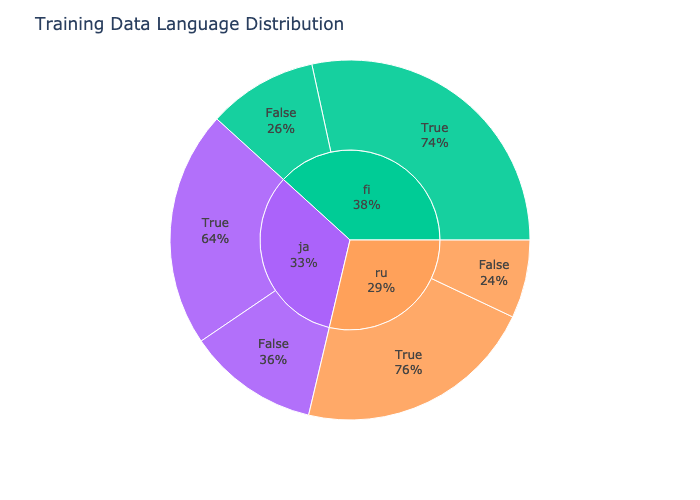
\includegraphics[width=0.8\textwidth]{../week1/plots/week1_a_dataset.png}
        \caption{Distribution of labels in the dataset}
        \label{fig:label_distribution}
    \end{figure}

    \begin{figure}[h]
        \centering
        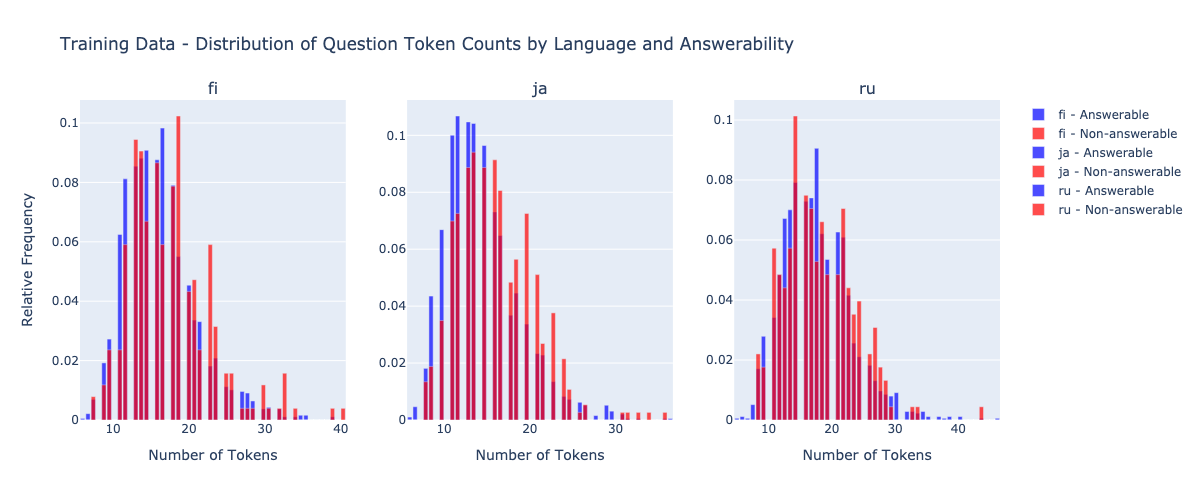
\includegraphics[width=0.8\textwidth]{../week1/plots/week1_a_lang_token_distribution_normalized.png}
        \caption{normalized Histogram for token count(using llama3 tokenizer) of answerable/unanswerable questions in the dataset}
        \label{fig:language_distribution}
    \end{figure}

    % (b) For each of the languages Finnish, Japanese and Russian, report the 5 most common 
    % words in the questions from the training set. What kind of words are they?
    \item[(b)] 

    \begin{lstlisting}[language=Python]
    import MeCab
    def get_top_words(df: pd.DataFrame, lang: str, n=5):
        df_lang = df[df['lang'] == lang].copy()
        
        if lang == 'ja':
            mecab = MeCab.Tagger("-Owakati")  # Initialize MeCab tokenizer
            df_lang.loc[:, 'words_question_tokens'] = df_lang['question'].apply(lambda x: mecab.parse(x).split())
        else:
            df_lang.loc[:, 'words_question_tokens'] = df_lang['question'].apply(lambda x: x.split(' '))
        
        all_tokens = np.concatenate(df_lang['words_question_tokens'].values)
        unique, counts = np.unique(all_tokens, return_counts=True)
        sorted_indices = np.argsort(counts)[::-1]
        top_unique_tokens = unique[sorted_indices][:n]
        top_tokens_dict = {token: int(count) for token, count in zip(top_unique_tokens, counts[sorted_indices][:n])}
        return top_tokens_dict
    \end{lstlisting}


    we get the following results:

    \begin{figure}[h]
        \centering
        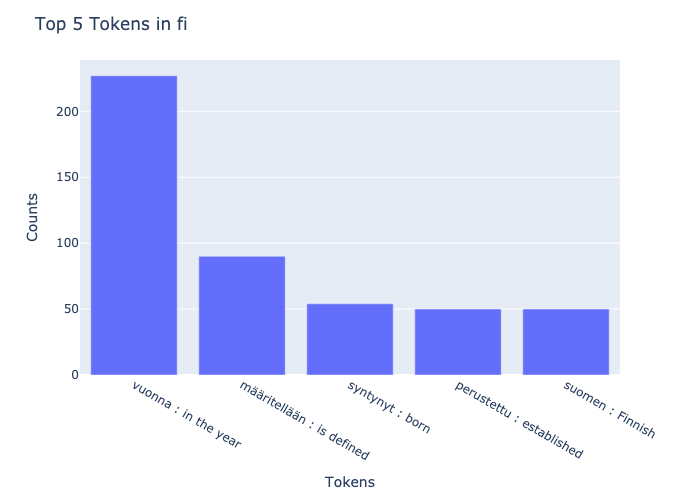
\includegraphics[width=0.8\textwidth]{../week1/plots/week1_b_top_5_tokens_fi.png}
        \caption{Top 5 tokens in Finnish}
        \label{fig:top_5_tokens_fi}
    \end{figure}

    \begin{figure}[h]
        \centering
        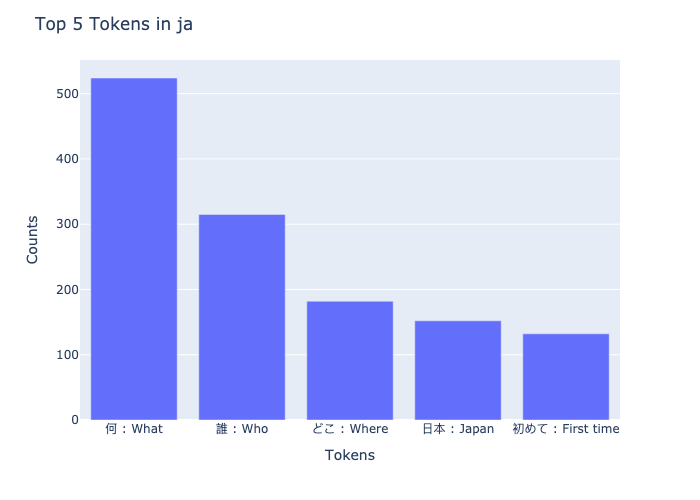
\includegraphics[width=0.8\textwidth]{../week1/plots/week1_b_top_5_tokens_ja.png}
        \caption{Top 5 tokens in Japanese}
        \label{fig:top_5_tokens_ja}
    \end{figure}

    \begin{figure}[h]
        \centering
        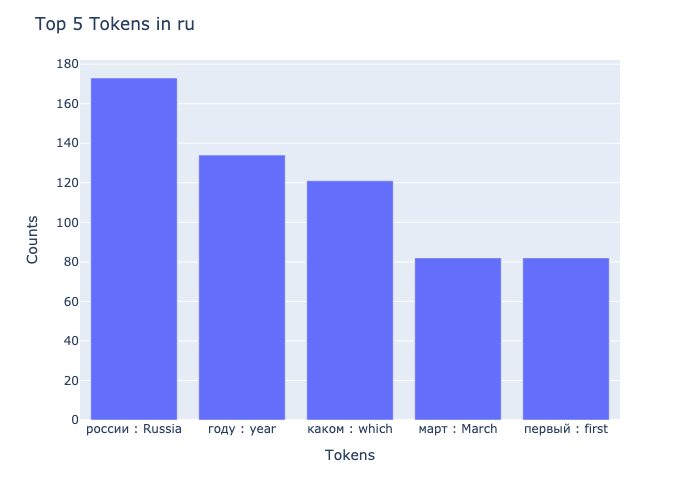
\includegraphics[width=0.8\textwidth]{../week1/plots/week1_b_top_5_tokens_ru.png}
        \caption{Top 5 tokens in Russian}
        \label{fig:top_5_tokens_ru}
    \end{figure}

% (c) Implement a rule-based classifier that predicts whether a question is answerable 
% or impossible, only using the document (context) and question. You may use machine 
% translation as a component. Use the answerable field to evaluate it on the validation set. 
% What is the performance of your classifier for each of the languages Finnish, Japanese and Russian?
    \item[(c)] 
\end{enumerate}

\section{Week 37 (9--15 September)}
% Let k be the number of members in your group (k ∈ {1, 2, 3}). Implement k different 
% language models for the questions in the three languages Finnish, Japanese and Russian, 
% as well as for the document contexts in English (total k × 4 language models), using the 
% training data. Evaluate each of them on the validation data, report their performance 
% and discuss the results.

\section{Week 38 (16--22 September)}
% Let k be the number of members in your group. For each of the three languages Finnish, 
% Japanese and Russian separately, using the training data, train k different classifiers 
% that receive the document (context) and question as input and predict whether the question 
% is answerable or impossible given the context. Evaluate the classifiers on the respective 
% validation sets, report and analyse the performance for each language and compare the 
% scores across languages.

\section{Week 39 (23--29 September)}
% Let k be the number of members in your group. Using the training data in Finnish, Japanese 
% and Russian separately, train k different sequence labellers, which predict the tokens in 
% a document context that constitute the answer to the corresponding question. You can decide 
% whether to train one model per language or a single model for all three languages. Evaluate 
% using a sequence labelling metric on the validation set, report and analyse the performance 
% for each language and compare the scores across languages.

\section{Week 40 (30 September--6 October)}
% Use the subset of the questions in Finnish, Japanese and Russian to train (or fine-tune) 
% an encoder-decoder model that receives the question and context as input and generates 
% the in-language answer. You can decide whether to train one model per language or a 
% single model for all three languages.

\section{Week 41+ (from 7 October)}
% Use all questions in Finnish, Japanese and Russian to train (or fine-tune) an encoder-decoder 
% model that receives the question and context as input and generates the English answer. 
% You can decide whether to train one model per question language or a single model for all 
% three languages. Evaluate using a text generation metric on the validation set, and compare 
% the overall results between answerable and unanswerable examples.

\end{document}